

\section*{\huge{Supplemental Information}}

\renewcommand{\thefigure}{S\arabic{figure}}
\renewcommand{\theequation}{S\arabic{equation}}
\renewcommand{\thetable}{S\arabic{table}}
\setcounter{equation}{0}
\setcounter{figure}{0}
\setcounter{table}{0}


% Note: this should go into a separate document eventually

\section*{Matrix derivatives in quantitative genetics equations}

As in the main text, $^{\textrm{T}}$ indicates transposition,
multiplication between matrices is always matrix multiplication, and
bold face indicates a matrix.
Also note that both $\mathbf{C}$ and $\mathbf{D}$ are symmetrical,
so $\mathbf{C} + \mathbf{C}^{\textrm{T}} = 2 \; \mathbf{C}$ and
$\mathbf{D} + \mathbf{D}^{\textrm{T}} = 2 \; \mathbf{D}$.


We can combine the equations in the Methods section as such:

\begin{equation} \label{eq:fitness-full}
\begin{split}
    F_{i,t+1} &= \exp \left\{
        r_0 - f \; \mathbf{v}_{i,t}^{\textrm{T}} \; \mathbf{C} \; \mathbf{v}_{i,t} -
        \alpha_0 \;\textrm{e}^{- \mathbf{v}_{i,t}^{\textrm{T}} \mathbf{v}_{i,t} } \bm{\Omega}_{i,t}
        \right\} \\
        \bm{\Omega}_{i,t} &\equiv N_{i,t} +
            \sum_{j \ne i}^{n}{ N_{j,t} \textrm{e}^{
            - \mathbf{v}_{j,t}^{\textrm{T}}
            \mathbf{D} \mathbf{v}_{j,t} } }
        \textrm{.}
\end{split}
\end{equation}

\noindent where $\bm{\Omega}_i$ represents the community abundance scaled
for the effect other species' axes values has on competition
experienced by species $i$.
Hereafter we will refer to $\bm{\Omega}_i$ as the scaled community size.




\subsection*{Axis evolution}

From the main text and above, we know that

\begin{equation}\label{eq:main-text-info-axis-change}
\begin{split}
    F_{i,t+1} &= \exp \left\{
        r_0 - f \; \mathbf{v}_{i,t}^{\textrm{T}} \; \mathbf{C} \; \mathbf{v}_{i,t} -
        \alpha_0 \;\textrm{e}^{- \mathbf{v}_{i,t}^{\textrm{T}} \mathbf{v}_{i,t} } \bm{\Omega}_{i,t}
        \right\} \\
    \mathbf{v}_{i,t+1} &= \mathbf{v}_{i,t} + \left( \frac{1}{F_{i,t+1}}
        \frac{\partial F_{i,t+1}}{\partial \mathbf{v}_{i,t}} \right) \sigma^2_i
    \textrm{.}
\end{split}
\end{equation}


The partial derivative of fitness in relation to axes for species $i$ is


\begin{equation*}
\begin{split}
    \frac{\partial F_{i,t+1}}{\partial \mathbf{v}_{i,t}} &=
        \exp \left\{
            r_0
            - f \mathbf{v}_{i,t}^{\textrm{T}} \mathbf{C} \mathbf{v}_{i,t}
            - \alpha_0  \bm{\Omega}_{i,t} \,
                \textrm{e}^{- \mathbf{v}_{i,t}^{\textrm{T}} \mathbf{v}_{i,t}}
        \right\}
        \frac{\partial \!
            \left(
                r_0
                - f \; \mathbf{v}_{i,t}^{\textrm{T}} \; \mathbf{C} \; \mathbf{v}_{i,t}
                - \alpha_0 \; \bm{\Omega}_{i,t} \;
                    \textrm{e}^{- \mathbf{v}_{i,t}^{\textrm{T}} \mathbf{v}_{i,t}}
            \right)
            }{ \partial \mathbf{v}_{i,t} } \\
     &=
        \exp \left\{
            r_0
            - f \mathbf{v}_{i,t}^{\textrm{T}} \mathbf{C} \mathbf{v}_{i,t}
            - \alpha_0  \bm{\Omega}_{i,t} \,
                \textrm{e}^{- \mathbf{v}_{i,t}^{\textrm{T}} \mathbf{v}_{i,t}}
        \right\}
        \left[
            - 2 f \mathbf{v}_{i,t}^{\textrm{T}} \mathbf{C}
            - \alpha_0 \, \bm{\Omega}_{i,t} \,
                \textrm{e}^{- \mathbf{v}_{i,t}^{\textrm{T}} \mathbf{v}_{i,t} } \:
                \frac{\partial \! \left( - \mathbf{v}_{i,t}^{\textrm{T}} \mathbf{v}_{i,t} \right)
                    }{ \partial \mathbf{v}_{i,t} }
        \right] \\[2ex]
    \frac{ \partial F_{i,t} }{ \partial \mathbf{v}_{i,t} } &=
        \exp \left\{
            r_0
            - f \mathbf{v}_{i,t}^{\textrm{T}} \mathbf{C} \mathbf{v}_{i,t}
            - \alpha_0  \bm{\Omega}_{i,t} \,
                \textrm{e}^{- \mathbf{v}_{i,t}^{\textrm{T}} \mathbf{v}_{i,t}}
        \right\}
        \left[
            2 \alpha_0 \bm{\Omega}_{i,t} \,
                \textrm{e}^{- \mathbf{v}_{i,t}^{\textrm{T}} \mathbf{v}_{i,t}} \:
                \mathbf{v}_{i,t}^{\textrm{T}}
            - 2 f \mathbf{v}_{i,t}^{\textrm{T}} \mathbf{C}
        \right]
    \textrm{.}
\end{split}
\end{equation*}



Combining above with equation \ref{eq:main-text-info-axis-change}, we find that axis values at
time $t+1$ are

\begin{equation} \label{eq:supp-axis-change-full}
    \mathbf{v}_{i,t+1} = \mathbf{v}_{i,t} + 2 \sigma_i^2
    \left(
        \alpha_0 \, \bm{\Omega}_{i,t} \:
            \textrm{e}^{- \mathbf{v}_{i,t}^{\textrm{T}} \mathbf{v}_{i,t}} \:
            \mathbf{v}_{i,t}^{\textrm{T}}
        - f \, \mathbf{v}_{i,t}^{\textrm{T}} \: \mathbf{C}
    \right)
    \textrm{.}
\end{equation}


\subsection*{Jacobian matrix}

The $n(q+1) \times n(q+1)$ Jacobian matrix consists of 

\begin{itemize}
\item $n^2$ blocks of size $q \times q$ containing
    $\partial \mathbf{v}_{i,t+1} / \partial \mathbf{v}_{\zeta,t}$
\item $n^2$ blocks of size $1 \times q$ containing
    $\partial \mathbf{v}_{i,t+1} / \partial N_{\zeta,t}$
\item $n^2$ blocks of size $q \times 1$ containing
    $\partial N_{i,t+1} / \partial \mathbf{v}_{\zeta,t}$
\item $n^2$ blocks of size $1 \times 1$ containing
    $\partial N_{i,t+1} / \partial N_{\zeta,t}$
\end{itemize}


for all $i \in \{ 1, \: \ldots \, , \: n \}$
and $\zeta \in \{ 1, \: \ldots \, , \: n \}$.


The partial derivatives of species $i$ axes at time $t+1$ with respect
to species $i$ axes at time $t$ are

\begin{equation*}
\begin{split}
    \frac{ \partial \, \mathbf{v}_{i,t+1} }{ \partial \, \mathbf{v}_{i,t} } &=
        \frac{ \partial \, \mathbf{v}_{i,t} }{ \partial \, \mathbf{v}_{i,t} } +
        2 \; \sigma_i^2
        \left(
            \frac{ \partial \;
                \alpha_0 \; \bm{\Omega}_{i,t} \;
                    \textrm{e}^{-\mathbf{v}_{i,t}^{\textrm{T}} \mathbf{v}_{i,t}} \,
                    \mathbf{v}_{i,t}^{\textrm{T}}}{\partial \; \mathbf{v}_{i,t} } -
            \frac{ \partial \; f \, \mathbf{v}_{i,t}^{\textrm{T}} \mathbf{C}}{\partial \; \mathbf{v}_{i,t} }
        \right) \\
    &=
        \mathbf{I} +
        2 \; \sigma_i^2
        \left[
            \alpha_0 \; \bm{\Omega}_{i,t} \,
            \left(
                \textrm{e}^{-\mathbf{v}_{i,t}^{\textrm{T}} \mathbf{v}_{i,t}} +
                \frac{ \partial \;
                        \textrm{e}^{-\mathbf{v}_{i,t}^{\textrm{T}} \mathbf{v}_{i,t}}
                        }{\partial \; \mathbf{v}_{i,t} } \, \mathbf{v}_{i,t}^{\textrm{T}}
            \right) -
            f \, \mathbf{C}^{\textrm{T}}
            \right] \\[2ex]
    \frac{ \partial \, \mathbf{v}_{i,t+1} }{ \partial \, \mathbf{v}_{i,t} } &= \mathbf{I} + 2 ~ \sigma_i^2 ~
        \left[
            \alpha_0 ~ \bm{\Omega}_{i,t} ~ \textrm{e}^{ - \mathbf{v}_{i,t}^{\textrm{T}} \mathbf{v}_{i,t} }
            \left(
                \mathbf{I} - 2 ~ \mathbf{v}_{i,t} \mathbf{v}_{i,t}^{\textrm{T}}
            \right) -
            f \: \mathbf{C}^{\textrm{T}}
        \right]
    \textrm{,}
\end{split}
\end{equation*}

\noindent where $\mathbf{I}$ is a $q \times q$ identity matrix.


Next we have the partial derivatives of species $i$ axes at time $t+1$ with respect to 
species $k$ axes at time $t$, where $k \ne i$.
To calculate this, it's useful to rearrange equation \ref{eq:axes-change-full} and
extract the portion that includes $\mathbf{v}_{k,t}$:


\begin{equation*}
\begin{split}
    \mathbf{v}_{i,t+1} &= \mathbf{v}_{i,t} + 2 \; \sigma_i^2
    \left[
        \left(
            N_{k,t} \; \textrm{e}^{ -\mathbf{v}_{k,t}^{\textrm{T}} \mathbf{D}
            \mathbf{v}_{k,t} } + \mathbf{\Phi}_{i,t}
        \right)
        \left(
            \alpha_0 \; \textrm{e}^{-\mathbf{v}_{i,t}^{\textrm{T}}
            \mathbf{v}_{i,t} } \; \mathbf{v}_{i,t}^{\textrm{T}}
        \right)
        - f \: \mathbf{v}_{i,t}^{\textrm{T}} \mathbf{C}
    \right] \\
    \mathbf{\Phi}_{i,t} &= N_{i,t} + \sum_{j \ne i, j \ne k}^{n}{
        N_{j,t} \; \textrm{e}^{- \mathbf{v}_{j,t}^{\textrm{T}}
        \mathbf{D} \mathbf{v}_{j,t} } }
    \textrm{.}
\end{split}
\end{equation*}

From this we calculated the partial derivative of $\mathbf{v}_{i,t+1}$ in relation to
$\mathbf{v}_{k,t}$


\begin{equation*}
\begin{split}
    \frac{ \partial \: \mathbf{v}_{i,t+1} }{ \partial \: \mathbf{v}_{k,t} } &=
        \frac{ \partial \: \mathbf{v}_{i,t} }{ \partial \: \mathbf{v}_{k,t} } +
        2 \; \sigma_i^2 \;
        \left[
            \frac{ \partial \:
                \left(
                    N_{k,t} \textrm{e}^{- \mathbf{v}_{k,t}^{\textrm{T}} \mathbf{D}
                    \mathbf{v}_{k,t}} + \mathbf{\Phi}_{i,t}
                \right)
                \left(
                    \alpha_0 \; \textrm{e}^{ - \mathbf{v}_{i,t}^{\textrm{T}}
                    \mathbf{v}_{i,t} } \mathbf{v}_{i,t}^{\textrm{T}}
                \right)
            }{ \partial \:  \mathbf{v}_{k,t} } -
            \frac{ \partial \:  f \, \mathbf{v}_{i,t}^{\textrm{T}} \mathbf{C} }{
            \partial \: \mathbf{v}_{k,t} }
        \right] \\
    &= 2 \; \sigma_i^2 \; \alpha_0 \; N_{k,t} \; \mathbf{v}_{i,t} \;
        \textrm{e}^{ - \mathbf{v}_{i,t}^{\textrm{T}}
        \mathbf{v}_{i,t} } \; 
        \frac{ \partial \:
                \textrm{e}^{
                    - \mathbf{v}_{k,t}^{\textrm{T}} \mathbf{D} \mathbf{v}_{k,t}
                    }
            }{ \partial \:  \mathbf{v}_{k,t} } \\
    &= 2 \; \sigma_i^2 \; \alpha_0 \; N_{k,t} \; \mathbf{v}_{i,t} \;
        \textrm{e}^{
                    - \mathbf{v}_{k,t}^{\textrm{T}} \mathbf{D} \mathbf{v}_{k,t}
                    - \mathbf{v}_{i,t}^{\textrm{T}} \mathbf{v}_{i,t}
                } \;
        \left[ 
            - 2 \, \mathbf{v}_{k,t}^{\textrm{T}} \, \mathbf{D}
        \right] \\
    \frac{ \partial \: \mathbf{v}_{i,t+1} }{ \partial \: \mathbf{v}_{k,t}} &=
        -4 \; \sigma_i^2 \; \alpha_0 \; N_{k,t} \; \mathbf{v}_{i,t} \;
        \textrm{e}^{
                    - \mathbf{v}_{k,t}^{\textrm{T}} \mathbf{D} \mathbf{v}_{k,t}
                    - \mathbf{v}_{i,t}^{\textrm{T}} \mathbf{v}_{i,t}
                } \;
        \mathbf{v}_{k,t}^{\textrm{T}} \; \mathbf{D}
    \textrm{.} \\
\end{split}
\end{equation*}

The partial derivatives of species $i$ axes in relation to species $i$ 
and species $k$ abundances are

\begin{equation*}
\begin{split}
    \frac{ \partial \: \mathbf{v}_{i,t+1} }{ \partial \: N_{i,t} } &=
        2 \; \sigma_i^2 \; \alpha_0 \; \mathbf{v}_{i,t} \;
        \textrm{e}^{ - \mathbf{v}_{i,t}^{\textrm{T}} \mathbf{v}_{i,t} } \\
    \frac{ \partial \: \mathbf{v}_{i,t+1} }{ \partial \: N_{k,t} } &=
        2 \; \sigma_i^2 \; \alpha_0 \; \mathbf{v}_{i,t} \;
        \textrm{e}^{ - \mathbf{v}_{k,t}^{\textrm{T}} \mathbf{D} \mathbf{v}_{k,t}
            - \mathbf{v}_{i,t}^{\textrm{T}} \mathbf{v}_{i,t} }
    \textrm{.} \\
\end{split}
\end{equation*}




For partial derivatives of abundances in relation to the other state variables,
we use the following equations from above:


\begin{equation*}
\begin{split}
    N_{i,t+1} &= N_{i,t} \; F_{i,t+1} \\
    F_{i,t+1} &=  \exp \left\{
        r_0 - f \, \mathbf{v}_{i,t}^{\text{T}} \, \mathbf{C} \, \mathbf{v}_{i,t} - 
        \alpha_0 \, \text{e}^{-\mathbf{v}_{i,t}^{\text{T}} \, \mathbf{v}_{i,t}} \,
        \Omega_{i,t}
    \right\} \\
    \Omega_{i,t} &= N_{i,t} + \sum_{j \ne i}^{n}{ N_j \:
        \text{e}^{- \mathbf{v}_{j,t}^{\text{T}} \, \mathbf{D} \, \mathbf{v}_{j,t} } }
    \textrm{.} \\
\end{split}
\end{equation*}



Using these, we have the following derivatives of abundances in relation
to axes:

\begin{equation*}
\begin{split}
    \frac{ \partial N_{i,t+1} }{ \partial \mathbf{v}_{i,t} } &= 
        2 \, F_{i,t+1} \,  N_{i,t}
        \left(
            \alpha_0 \, \Omega_{i,t} \, \text{e}^{ -\mathbf{v}_{i,t}^{\text{T}}
            \mathbf{v}_{i,t} } \, \mathbf{v}_{i,t}^{\text{T}}
            - f \, \mathbf{v}_{i,t}^{\text{T}} \, \mathbf{C}
        \right) \\
    \frac{ \partial N_{i,t+1} }{ \partial \mathbf{v}_{k,t} } &= 
        2 \, F_{i,t+1} \, N_{i,t} \, N_{k,t} \, \alpha_0 \: 
        \text{e}^{ -\mathbf{v}_{i,t}^{\text{T}} \mathbf{v}_{i,t} -
            \mathbf{v}_{k,t}^{\text{T}} \mathbf{D} \mathbf{v}_{k,t} } \:
        \mathbf{v}_{k,t}^{\text{T}} \, \mathbf{D}
    \textrm{.}
\end{split}
\end{equation*}

We also have the following derivatives of abundances at time $t+1$ in relation
to those at time $t$:

\begin{equation*}
\begin{split}
    \frac{ \partial N_{i,t+1} }{ \partial N_{i,t} } &= 
        F_{i,t+1}
        \left(
            1 - N_{i,t} \: \alpha_0 \: 
            \text{e}^{ -\mathbf{v}_{i,t}^{\text{T}} \mathbf{v}_{i,t} } 
        \right) \\
    %
    \frac{ \partial N_{i,t+1} }{ \partial N_{k,t} } &= 
        - F_{i,t+1} \: N_{i,t} \: \alpha_0 \: 
        \text{e}^{ -\mathbf{v}_{i,t}^{\text{T}} \mathbf{v}_{i,t} -
            \mathbf{v}_{k,t}^{\text{T}} \mathbf{D} \mathbf{v}_{k,t} } 
    \textrm{.}
\end{split}
\end{equation*}











% ========================================================================================
% ========================================================================================
% ========================================================================================
% ========================================================================================
% ========================================================================================
% ========================================================================================
% ========================================================================================






\section*{Two-axis equilibrium solutions}

For these solutions, we will no longer use matrix notation.
Also, since all axes have the same costs, benefits, and
non-additive effects, solutions for axis 1 and 2 are the same.
Only solutions for axis 1 are presented.
We use a hat to distinguish equilibrium values
($\hat{Z}$ for parameter $Z$).
Lastly, because $\mathbf{C}$ is symmetrical, only has 2 rows and columns, and
differs only on the off-diagonals, there is only one $\eta$ value.


\subsection*{Axis values}

The two axes for species $i$ change as follows:

\begin{equation*}
\begin{split}
    v_{i1,t+1} &= v_{i1,t} + 2 \; \sigma^2
    \left[
        \alpha_0 \; \Omega_{i,t} \;
            \textrm{e}^{-v_{i1,t}^2 - v_{i2,t}^2} \; v_{i1,t}
        - f \; ( v_{i1,t} + \eta \; v_{i2,t} )
    \right] \\
    v_{i2,t+1} &= v_{i2,t} + 2 \; \sigma^2
    \left[
        \alpha_0 \; \Omega_{i,t} \;
            \textrm{e}^{-v_{i2,t}^2 - v_{i1,t}^2} \; v_{i2,t}
        - f \; ( v_{i2,t} + \eta \; v_{i1,t} )
    \right] \\
    \Omega_{i,t} &\equiv N_{i,t} +
        \sum_{j \ne i}^{n}{ N_{j,t} \; \textrm{e}^{
                - d_1 v_{j1,t}^2 - d_2 v_{j2,t}^2 } }
    \textrm{.}
\end{split}
\end{equation*}


We'll now drop indices for species and time because we are
focusing on just one species and time point.



At equilibrium (assuming that $\sigma > 0$),

\begin{equation}
\begin{split}
    0 &= \alpha_0 \; \hat{\Omega} \;
            \textrm{e}^{-\hat{v}_{1}^2 - \hat{v}_{2}^2} \; \hat{v}_{1}
        - f \; ( \hat{v}_{1} + \eta \; \hat{v}_{2} ) \\
    0 &=
        \alpha_0 \; \hat{\Omega} \;
            \textrm{e}^{-\hat{v}_{2}^2 - \hat{v}_{1}^2} \; \hat{v}_{2}
        - f \; ( \hat{v}_{2} + \eta \; \hat{v}_{1} )
    \textrm{.}
\end{split}
\label{eq:two-axes-v-eq1}
\end{equation}


\noindent Thus, we have

\begin{equation*}
\begin{split}
    \alpha_0 \; \hat{\Omega} \; \textrm{e}^{-\hat{v}_{1}^2 - \hat{v}_{2}^2} &=
        \frac{ f \; ( \hat{v}_{1} + \eta \; \hat{v}_{2} ) }{ \hat{v}_{1} } \\
    \alpha_0 \; \hat{\Omega} \; \textrm{e}^{-\hat{v}_{1}^2 - \hat{v}_{2}^2} &=
        \frac{ f \; ( \hat{v}_{2} + \eta \; \hat{v}_{1} ) }{ \hat{v}_{2} }
    \textrm{.}
\end{split}
\end{equation*}


\noindent Combining these leads to

\begin{equation*}
\begin{split}
    f \; ( \hat{v}_{1} + \eta \; \hat{v}_{2} ) \; \hat{v}_{2} &=
        f \; ( \hat{v}_{2} + \eta \; \hat{v}_{1} ) \; \hat{v}_{1} \\
    f \hat{v}_{1} \hat{v}_{2} + \eta \hat{v}_{2}^2 &=
        f \hat{v}_{1} \hat{v}_{2} + \eta \hat{v}_{1}^2 \\
    \eta \hat{v}_{2}^2 &= \eta \hat{v}_{1}^2 \\
    \hat{v}_{1} &= \hat{v}_{2}
    \textrm{.}
\end{split}
\end{equation*}

Since all $v$ must be $\ge 0$ (hence no $\pm$ in the equation above),
either $\hat{v}_{1} = \hat{v}_{2}$ or not (when $\eta = 0$).
Plugging in $\hat{v}_{1} = \hat{v}_{2}$ into equation \ref{eq:two-axes-v-eq1}
gives us

\begin{equation*}
\begin{split}
    0 &= \alpha_0 \; \hat{\Omega} \; \textrm{e}^{-2 \; \hat{v}_{1}^2 } \; \hat{v}_{1}
        - f \; ( \hat{v}_{1} + \eta \; \hat{v}_{1} ) \\
    &= \hat{v}_{1} \left[ \alpha_0 \; \hat{\Omega} \; \textrm{e}^{-2 \; \hat{v}_{1}^2 }
        - f \; ( 1 + \eta ) \right]
    \textrm{.}
\end{split}
\end{equation*}

\noindent One solution is $\hat{v}_{1} = 0$, but if $\hat{v}_{1} \ne 0$


\begin{equation}
\begin{split}
    \alpha_0 \; \hat{\Omega} \; \textrm{e}^{-2 \; \hat{v}_{1}^2 } &=
        f \; ( 1 + \eta ) \\
    -2 \; \hat{v}_{1}^2 &=
        \log \left( \frac{ f \; ( 1 + \eta ) }{ \alpha_0 \; \hat{\Omega} } \right) \\
    \hat{v}_{1} &= \sqrt{\frac{1}{2}
        \log \left( \frac{ \alpha_0 \; \hat{\Omega} }{ f \; ( 1 + \eta ) } \right) }
    \textrm{.}
\end{split}
\label{eq:two-axes-v-eq5}
\end{equation}



When $\eta = 0$ and at least one of the two axes $\ne 0$,
axes are constrained by their distance
from the origin: $\sqrt{\hat{v}_{1}^2 + \hat{v}_{2}^2}$.
When $\hat{v}_{1} \ne 0$, this distance is

\begin{equation*}
\begin{split}
    0 &= \alpha_0 \; \hat{\Omega} \;
            \textrm{e}^{-\hat{v}_{1}^2 - \hat{v}_{2}^2} \; \hat{v}_{1}
        - f \; \hat{v}_{1} \\
    0 &= \alpha_0 \; \hat{\Omega} \;
        \textrm{e}^{- ( \hat{v}_{1}^2 + \hat{v}_{2}^2) }
        - f \\
    \log \left( \frac{\alpha_0 \; \hat{\Omega}}{ f } \right) &=
        \hat{v}_{1}^2 + \hat{v}_{2}^2 \\
     \sqrt{ \hat{v}_{1}^2 + \hat{v}_{2}^2 } &=
        \sqrt{ \log \left( \frac{\alpha_0 \; \hat{\Omega}}{ f } \right)}
    \textrm{.}
\end{split}
\end{equation*}

\noindent So the relationship between axes when $\eta = 0$ is

$$
    \hat{v}_{1} =
    \sqrt{
        \log \left( \frac{\alpha_0 \; \hat{\Omega}}{ f } \right) -
        \hat{v}_{2}^2
    }
    \textrm{,}
$$

\noindent when $\hat{v}_{2}^2 \ge \log (\alpha_0 \hat{\Omega} / f)$.

We've shown solutions for when $v_1 = v_2$ and when $\eta = 0$, but
when one axis is zero but the other is not (and $\eta$ isn't necessarily 0),
we get the following (for $v_1 \ne 0$ and $v_2 = 0$):

\begin{equation}
\begin{split}
    0 &=
        \alpha_0 \; \hat{\Omega} \;
            \textrm{e}^{-\hat{v}_{1}^2 - \hat{v}_{2}^2} \; \hat{v}_{1}
        - f \; ( \hat{v}_{1} + \eta \; \hat{v}_{2} ) \\
    0 &=
        \alpha_0 \; \hat{\Omega} \;
            \textrm{e}^{-\hat{v}_{1}^2} \; \hat{v}_{1}
        - f \; \hat{v}_{1} \\
    0 &=
        \alpha_0 \; \hat{\Omega} \;
            \textrm{e}^{-\hat{v}_{1}^2} - f \\
    \frac{f}{\alpha_0 \; \hat{\Omega}} &=
         \frac{1}{\textrm{e}^{\hat{v}_{1}^2}} \\
    \hat{v}_{1} &= \sqrt{ \log \left( \frac{\alpha_0 \; \hat{\Omega}}{f} \right) }
\end{split}
\label{eq:two-axes-v1-nonzero-v2-zero}
\end{equation}







% -----------------------------------------------------------------
% -----------------------------------------------------------------







\subsection*{Scaled community size}

Fitness for the species is written as

$$
    F = \exp \left\{
        r_0 - f ( {v}_{1}^2 + 2 \eta {v}_{1} {v}_{2} + {v}_{2}^2 ) -
        \alpha_0 \, \textrm{e}^{ - {v}_{1}^2 - {v}_{2}^2 } \, \Omega
    \right\}
    \textrm{.}
$$


\noindent At equilibrium,

\begin{equation}
    0 = r_0 - f ( \hat{v}_{1}^2 + 2 \eta \hat{v}_{1} \hat{v}_{2} + \hat{v}_{2}^2 ) -
        \alpha_0 \, \textrm{e}^{ - {v}_{1}^2 - {v}_{2}^2 } \, \Omega
    \textrm{.}
\label{eq:two-axes-omega-equil-start}
\end{equation}


\noindent When $\hat{v}_1 = \hat{v}_2$, we can insert our answer from
\ref{eq:two-axes-v-eq5} to get

\begin{equation*}
\begin{split}
    0 &= r_0 - 2 \; f \; \hat{v}_{1}^2 ( 1 + \eta ) -
        \alpha_0 \textrm{e}^{ -2 \; \hat{v}_{1}^2 } \hat{\Omega} \\
    r_0 &= 2 f ( 1 + \eta ) \left[
        \frac{1}{2}
        \log \left( \frac{ \alpha_0 \; \hat{\Omega} }{ f \; ( 1 + \eta ) } \right)
    \right] +
        \alpha_0 \textrm{e}^{ -2 \;
            \left[
                \frac{1}{2} \log \left(
                    \frac{ \alpha_0 \; \hat{\Omega} }{ f \; ( 1 + \eta ) }
                \right)
            \right]
        } \hat{\Omega} \\
    r_0 &= f ( 1 + \eta ) \log \left(
        \frac{ \alpha_0 \; \hat{\Omega} }{ f \; ( 1 + \eta ) }
    \right) + f ( 1 + \eta ) \\
    \frac{  r_0 - f ( 1 + \eta ) }{ f ( 1 + \eta ) } &=
        \log \left(
        \frac{ \alpha_0 \; \hat{\Omega} }{ f \; ( 1 + \eta ) }
        \right) \\
    \hat{\Omega} &= \frac{ f \; ( 1 + \eta ) }{ \alpha_0 } \;
        \textrm{e}^{\frac{  r_0 }{ f ( 1 + \eta ) } - 1 }
    \textrm{.}
\end{split}
\end{equation*}

Thus, when $\hat{v}_1 = \hat{v}_2$,
$$
\hat{\Omega} = \frac{ f \; ( 1 + \eta ) }{ \alpha_0 } \;
        \textrm{e}^{\frac{ r_0 }{ f ( 1 + \eta ) } - 1 }
    \textrm{.}
$$


\noindent When $\eta = 0$,

$$
    \hat{\Omega} = \frac{ f }{ \alpha_0 } \; \textrm{e}^{\frac{ r_0 }{ f } - 1 }
    \textrm{.}
$$



If instead $v_1 = 0$ and $v_2 \ne 0$, we can start by simplifying equation
\ref{eq:two-axes-omega-equil-start}

\begin{equation*}
\begin{split}
    0 &= r_0 - f \hat{v}_{1}^2 -
        \alpha_0 \textrm{e}^{ - \hat{v}_{1}^2 } \hat{\Omega} \\
    \hat{\Omega} &= \frac{ r_0 - f \hat{v}_{1}^2 }{ \alpha_0 } \textrm{e}^{ \hat{v}_{1}^2 }
    \textrm{.}
\end{split}
\end{equation*}

Now we combine this with \ref{eq:two-axes-v1-nonzero-v2-zero}

\begin{equation*}
\begin{split}
    \hat{\Omega} &= \frac{ r_0 - f \log \left( \frac{\alpha_0 \hat{\Omega}}{f} \right) }{
        \alpha_0 } \left( \frac{\alpha_0 \; \hat{\Omega}}{f} \right) \\
    1 &= \frac{ r_0 }{ f } - \log \left( \frac{\alpha_0 \hat{\Omega}}{f} \right) \\
    \hat{\Omega} &= \frac{f}{\alpha_0} \textrm{e}^{\frac{r_0}{f} - 1}
    \textrm{.}
\end{split}
\end{equation*}











% -----------------------------------------------------------------
% -----------------------------------------------------------------








\subsection*{Combined solutions}

When $\hat{v}_1 = \hat{v}_2$,

\begin{equation}  \label{eq:two-axes-finals-eta-negative}
\begin{split}
    \hat{\Omega} &= \frac{ f \; ( 1 + \eta ) }{ \alpha_0 } \;
        \textrm{e}^{\frac{  r_0 }{ f ( 1 + \eta ) } - 1 }
        \\
    \hat{v}_1 &= \sqrt{
        \frac{1}{2} \left( \frac{ r_0 }{ f (1 + \eta) } - 1 \right)
    }
    \textrm{.}
\end{split}
\end{equation}


\noindent When $\eta = 0$,

\begin{equation}  \label{eq:two-axes-finals-eta-zero}
\begin{split}
    \hat{\Omega} &= \frac{ f }{ \alpha_0 } \; \textrm{e}^{\frac{ r_0 }{ f } - 1 } \\
    \sqrt{\hat{v}_1^2 + \hat{v}_2^2} &= \sqrt{ \frac{ r_0 }{ f } - 1 } \\
    \hat{v}_1 &= \sqrt{ \frac{ r_0  }{ f } - \hat{v}_2^2 - 1 }
    \textrm{.}
\end{split}
\end{equation}


\noindent When $v_1 \ne 0$, $v_2 = 0$, and $\eta \ne 0$,

\begin{equation}  \label{eq:two-axes-finals-eta-positive}
\begin{split}
    \hat{\Omega} &= \frac{f}{\alpha_0} \textrm{e}^{\frac{r_0}{f} - 1} \\
    \hat{v}_1 &= \sqrt{ \frac{ r_0 }{ f } - 1 }
    \textrm{.}
\end{split}
\end{equation}

\noindent Thus, when $v_1 \ne 0$, $v_2 = 0$, and $\eta \ne 0$, the equilibrium
dynamics match that for when $\eta = 0$, which is not surprising given that
you cannot have a non-additive tradeoff when one axis has a zero value.









% -----------------------------------------------------------------
% -----------------------------------------------------------------








\subsection*{Differences in abundance among species}



This section analyzes a two-species community where each species has one of two potential
outcomes in terms of axis equilibria:
(1) $\hat{v}_1 = \hat{v}_2$ and
(2) $\hat{v}_1 \ne 0 \; \& \; \hat{v}_2 = 0$.
I'm not discussing when $\eta = 0$ because that's not biologically very realistic
and those results are likely an artifact of the model structure.


\subsubsection*{At the same axis equilibrium:}

The first scenario is when both species have $\hat{v}_1 = \hat{v}_2$.
If this is the case, then from above, we know that

\begin{equation*}
\begin{split}
    \hat{v}_{11} &= \hat{v}_{12} = \hat{v}_{21} = \hat{v}_{22} = \sqrt{\frac{1}{2}
        \left( \frac{r_0}{f (1 + \eta)} - 1 \right)} \\
    \hat\Omega_1 &= \hat\Omega_2 = \frac{f (1 + \eta)}{\alpha_0}
        \text{e}^{\frac{r_0}{f (1 + \eta)} - 1}
    \text{.}
\end{split}
\end{equation*}

Because all axes and scale community sizes are equal, and because of our
definition of $\Omega$ from equation ??
% \ref{eq:fitness-full}

\begin{equation} \label{eq:two-axes-v1-v2-equal-N1-N2}
\begin{split}
    \hat{N}_1 + \hat{N}_2 \: \text{e}^{-\hat{v}_{11}^2 (d_1 + d_2)} &=
        \hat{N}_2 + \hat{N}_1 \: \text{e}^{-\hat{v}_{11}^2 (d_1 + d_2)} \\
    \hat{N}_1 \left( 1 - \text{e}^{-\hat{v}_{11}^2 (d_1 + d_2)} \right) &=
        \hat{N}_2 \left( 1 - \text{e}^{-\hat{v}_{11}^2 (d_1 + d_2)} \right) \\
    \hat{N}_1 &= \hat{N}_2
    \text{.}
\end{split}
\end{equation}

\noindent Combining the above two sets of equations to solve for $\hat{N}_1$ in
terms of parameters:


\begin{equation} \label{eq:two-axes-v1-v2-equal-N}
\begin{split}
    \hat\Omega_1 &= \hat{N}_1 + \hat{N}_2 \: \text{e}^{-d_1 \hat{v}_{21}^2 -
        d_2 v_{22}^2} \\
    \frac{f (1 + \eta)}{\alpha_0} \text{e}^{\frac{r_0}{f (1 + \eta)} - 1} &=
        \hat{N}_1 + \hat{N}_1 \: \text{e}^{- \hat{v}_{11}^2 (d_1 + d_2)} \\
    \frac{f (1 + \eta)}{\alpha_0} \text{e}^{\frac{r_0}{f (1 + \eta)} - 1} &=
        \hat{N}_1 \left[ 1 + \text{e}^{- \frac{1}{2} \left(
            \frac{r_0}{f (1 + \eta)} - 1 \right) (d_1 + d_2)} \right] \\
    \hat{N}_1 &= \frac{f (1 + \eta)}{\alpha_0  \left[ 1 + \text{e}^{- \frac{1}{2} \left(
        \frac{r_0}{f (1 + \eta)} - 1 \right) (d_1 + d_2)} \right] } \;
        \text{e}^{\frac{r_0}{f (1 + \eta)} - 1}
    \text{.}
\end{split}
\end{equation}


This extends to $n$ species as follows:

\begin{equation} \label{eq:two-axes-v1-v2-equal-N-n-species}
    \hat{N}_1 = \frac{f (1 + \eta)}{\alpha_0  \left[ 1 + \text{e}^{- \frac{1}{2} \left(
        \frac{r_0}{f (1 + \eta)} - 1 \right) (d_1 + d_2)}  (n - 1) \right] } \;
        \text{e}^{\frac{r_0}{f (1 + \eta)} - 1}
    \text{.}
\end{equation}




Similarly, when both species have $\hat{v}_1 \ne 0 \; \& \; \hat{v}_2 = 0$:

\begin{equation*}
\begin{split}
    \hat{v}_{11} &= \hat{v}_{21} = \sqrt{ \frac{ r_0 }{ f } - 1 } \\
    \hat{v}_{12} &= \hat{v}_{22} = 0 \\
    \hat\Omega_1 &= \hat\Omega_2 = \frac{f}{\alpha_0} \textrm{e}^{\frac{r_0}{f} - 1}
    \text{.}
\end{split}
\end{equation*}

\noindent Therefore,

\begin{equation} \label{eq:two-axes-v1-nonzero-v2-zero-N1-N2}
\begin{split}
    \hat{N}_1 + \hat{N}_2 \: \text{e}^{- d_1 \hat{v}_{11}^2 } &=
        \hat{N}_2 + \hat{N}_1 \: \text{e}^{- d_1 \hat{v}_{11}^2 } \\
    \hat{N}_1 \left( 1 - \text{e}^{- d_1 \hat{v}_{11}^2 } \right) &=
        \hat{N}_2 \left( 1 - \text{e}^{- d_1 \hat{v}_{11}^2 } \right) \\
    \hat{N}_1 &= \hat{N}_2
    \text{.}
\end{split}
\end{equation}

\noindent And,

\begin{equation} \label{eq:two-axes-v1-nonzero-v2-zero-N}
\begin{split}
    \hat\Omega_1 &= \hat{N}_1 + \hat{N}_2 \: \text{e}^{-d_1 \hat{v}_{21}^2 -
        d_2 v_{22}^2} \\
    \frac{f}{\alpha_0} \textrm{e}^{\frac{r_0}{f} - 1} &= \hat{N}_1 \left[
        1 + \text{e}^{- d_1 \left( \frac{ r_0 }{ f } - 1 \right) } \right] \\
    \hat{N}_1 &= \frac{ f }{ \alpha_0 \left[ 1 + \text{e}^{- d_1 \left(
        \frac{ r_0 }{ f } - 1 \right) } \right] } \; \text{e}^{\frac{r_0}{f} - 1}
    \text{.}
\end{split}
\end{equation}


For $n$ species

\begin{equation} \label{eq:two-axes-v1-nonzero-v2-zero-N-n-species}
    \hat{N}_1 = \frac{ f }{ \alpha_0 \left[ 1 + \text{e}^{- d_1 \left(
        \frac{ r_0 }{ f } - 1 \right) } (n - 1) \right] } \; \text{e}^{\frac{r_0}{f} - 1}
    \text{.}
\end{equation}





% ----------------------------------------
% ----------------------------------------

\subsubsection*{At different axis equilibria:}




Now we'll look at what happens when the species differ in their axis equilibria.
If $\hat{v}_{11} = \hat{v}_{12}$ and $\hat{v}_{21} \ne 0 \; \& \; \hat{v}_{22} = 0$

\begin{equation*}
\begin{split}
    \hat{v}_{11} &= \hat{v}_{12} = \sqrt{\frac{1}{2}
        \left( \frac{r_0}{f (1 + \eta)} - 1 \right)} \\
    \hat{v}_{21} &= \sqrt{ \frac{ r_0 }{ f } - 1 } \\
    \hat{v}_{22} &= 0 \\
    \hat\Omega_1 &= \frac{f (1 + \eta)}{\alpha_0}
        \text{e}^{\frac{r_0}{f (1 + \eta)} - 1} \\
    \hat\Omega_2 &= \frac{f}{\alpha_0} \textrm{e}^{\frac{r_0}{f} - 1}
    \text{.}
\end{split}
\end{equation*}

Therefore,

\begin{equation*}
\begin{split}
    \frac{\hat\Omega_1}{\hat\Omega_2} &= \left[
            \frac{f (1 + \eta)}{\alpha_0}
            \text{e}^{\frac{r_0}{f (1 + \eta)} - 1}
        \right] \left[
            \frac{ \alpha_0 }{ f \; \textrm{e}^{\frac{r_0}{f} - 1} }
        \right] \\
    &= ( 1 + \eta) \text{e}^{\frac{ r_0 - r_0 \, (1 + \eta) }{f (1 + \eta)}} \\
    \hat\Omega_1 &= ( 1 + \eta) \; \text{e}^{\frac{ - r_0 \eta }{f (1 + \eta)}} \;
        \hat\Omega_2
    \text{.}
\end{split}
\end{equation*}


Now looking at the relationship between $\hat{N}_1$ and $\hat{N}_2$:

\begin{equation*}
\begin{split}
    \hat{N}_1 + \hat{N}_2 \; \text{e}^{-d_1 \left( \frac{r_0}{f} - 1 \right)} &=
        ( 1 + \eta) \; \text{e}^{\frac{ - r_0 \eta }{f (1 + \eta)}}
        \left[
            \hat{N}_2 + \hat{N}_1 \; \text{e}^{- \frac{1}{2}
            \left(
                \frac{r_0}{f (1 + \eta)} - 1
            \right) (d_1 + d_2)}
        \right] \\
    \hat{N}_1 + \hat{N}_2 \; \text{e}^{-d_1 \left( \frac{r_0}{f} - 1 \right)} &=
        \hat{N}_2 ( 1 + \eta) \; \text{e}^{\frac{ - r_0 \eta }{f (1 + \eta)}} +
        \hat{N}_1 \; \text{e}^{ - \frac{1}{2} (d_1 + d_2) \left(
            \frac{r_0 - f (1 + \eta)}{f (1 + \eta)} \right) -
            \left( \frac{r_0 \eta}{ f (1 + \eta) } \right)  } \\
    \hat{N}_1 &= \hat{N}_2 \frac{ ( 1 + \eta) \;
        \text{e}^{\frac{ - r_0 \eta }{f (1 + \eta)}} -
        \text{e}^{-d_1 \left( \frac{r_0}{f} - 1 \right)} }{
        1 - \text{e}^{ - \frac{1}{2 f (1 + \eta)} \left[ (d_1 + d_2)
        \left( r_0 - f (1 + \eta) \right) + 2 r_0 \eta \right]  } }
    \text{.}
\end{split}
\end{equation*}







% ========================================================================================
% ========================================================================================
% ========================================================================================
% ========================================================================================
% ========================================================================================
% ========================================================================================
% ========================================================================================


\section*{Effects of stochasticity on axis evolution}

From the main text, we know that when there is variability in axis evolution, 

\begin{equation*}
\begin{split}
    \mathbf{\ddot{v}}_{i,t+1} &= \mathbf{v}_{i,t+1} \; \text{e}^{\varepsilon_V} \\
    \varepsilon_V &\sim \text{N}(0, \, \sigma^2_V) \\
    \mathbf{v}_{i,t+1} &= \mathbf{v}_{i,t} + \left( \frac{1}{F_i}
        \frac{\partial F_i}{\partial \mathbf{\ddot{v}}_{i,t}} \right) \sigma^2_i
    \text{.}
\end{split}
\end{equation*}



For the two-axis case, we can define the function $G_1$ for axis 1 as a function 
of the random variables $\varepsilon_1$ and $\varepsilon_2$:

\begin{equation*}
    G_1(\varepsilon_1, \varepsilon_2) = v_{i1,t} + 2 \; \sigma_i^2
    \left[
        \alpha_0 \; \Omega_{i,t} \;
            \text{e}^{-(v_{i1,t} \text{e}^{\varepsilon_1})^2 - (v_{i2,t} \text{e}^{\varepsilon_2})^2} \; v_{i1,t} \text{e}^{\varepsilon_1}
        - f \; ( v_{i1,t} \text{e}^{\varepsilon_1} + \eta \; v_{i2,t} \text{e}^{\varepsilon_2} )
    \right]
\end{equation*}


The second order Taylor series approximation for $G_1(\varepsilon_1, \varepsilon_2)$,
about $\bm{\theta} = \{ \mu_{\varepsilon_1}, \mu_{\varepsilon_2} \} = \{ 0, 0 \}$, is

\begin{equation}
\label{eq:taylor-expansion-outline}
    \text{E}(G_1(\varepsilon_1, \varepsilon_2)) \approx G_1(\bm{\theta}) + 
        \frac{1}{2} \left[ 
            \left. \frac{\partial^2 G_1}{\partial^2 \varepsilon_1} \right\lvert_{\bm{\theta}} \; \sigma^2_{\varepsilon_1} +
            \left. \frac{\partial^2 G_1}{\partial^2 \varepsilon_2} \right\lvert_{\bm{\theta}} \; \sigma^2_{\varepsilon_2}
        \right]
\text{.}
\end{equation}


In the derivatives below, we have removed indices for species and time for clarity.
To avoid confusion in later equations, $\sigma_A^2$ is additive genetic variance.

We have the following derivatives of $G_1$ with respect to the random variables $\varepsilon_1$ and $\varepsilon_1$:

\begin{equation*}
\begin{split}
    \frac{\partial \, G_1}{\partial \, \varepsilon_1} &= 2 \; \sigma_A^2 \: v_{1} \: \text{e}^{\varepsilon_1}
    \left[
        \alpha_0 \; \Omega \;
            \text{e}^{-(v_{1} \: \text{e}^{\varepsilon_1})^2 - (v_{2} \: \text{e}^{\varepsilon_2})^2}
            \left(
                1 - 2 \, v_{1}^2 \: \text{e}^{2 \varepsilon_1}
            \right)
        - f
    \right] \\
% 
    \frac{\partial^2 G_1}{\partial^2 \varepsilon_1} &= 2 \; \sigma_A^2 \: v_{1} \: \text{e}^{\varepsilon_1}
    \left[
        \alpha_0 \; \Omega \;
            \text{e}^{-(v_{1} \: \text{e}^{\varepsilon_1})^2 - (v_{2} \: \text{e}^{\varepsilon_2})^2}
            \left(
                1 - 8 \, v_{1}^2 \: \text{e}^{2 \varepsilon_1}
            \right)
        - f
    \right] \\[2ex]
%
%
    \frac{\partial \, G_1}{\partial \, \varepsilon_2} &= - 2 \; \sigma_A^2
    \left[
        2 \: \alpha_0 \; \Omega \; v_1 \; v_2^2 \;
            \text{e}^{-(v_{1} \: \text{e}^{\varepsilon_1})^2 - (v_{2} \: \text{e}^{\varepsilon_2})^2 + \varepsilon_1 + 2 \, \varepsilon_2}
        + f \: \eta \: v_2 \: \text{e}^{\varepsilon_2}
    \right] \\
% 
    \frac{\partial^2 G_1}{\partial^2 \varepsilon_2} &= - 2 \; \sigma_A^2
    \left[
        4 \: \alpha_0 \; \Omega \; v_1 \; v_2^2 \;
            \text{e}^{-(v_{1} \: \text{e}^{\varepsilon_1})^2 - (v_{2} \: \text{e}^{\varepsilon_2})^2 + \varepsilon_1 + 2 \, \varepsilon_2}
            \left(
                1 - v_{2}^2 \: \text{e}^{2 \varepsilon_2}
            \right)
        + f \: \eta \: v_2 \: \text{e}^{\varepsilon_2}
    \right]
\text{.}
\end{split}
\end{equation*}


Combining these with equation \ref{eq:taylor-expansion-outline} give us 

\begin{equation*}
\begin{split}
    \text{E}(G_1(\varepsilon_1, \varepsilon_2)) \approx \; &
        v_1 + 2 \; \sigma_A^2 \left[ 
            \alpha_0 \; \Omega \; v_1 \; \text{e}^{-v_1^2 - v_2^2} - f (v_1 + \eta \; v_2)
        \right] \\
        &+ \frac{1}{2} \Bigg\{
            2 \; \sigma_A^2 \; v_1 \left[
                \alpha_0 \; \Omega \; \text{e}^{-v_1^2 - v_2^2} \left( 1 - 8 \; v_1^2 \right) - f
            \right] \sigma^2_{\varepsilon_1} \\
            & \hspace{2.5em} - 2 \; \sigma_A^2 \left[
                4 \; \alpha_0 \; \Omega \; v_1 \; v_2^2 \; \text{e}^{-v_1^2 - v_2^2} \left( 1 - v_2^2 \right) + f \; \eta \; v_2
            \right] \sigma^2_{\varepsilon_2}
        \Bigg\} %\\[2ex]
%
%
%    \approx ~ & v_1 + \sigma_A^2 \Big[ 
%            2 \alpha_0 \Omega v_1 \text{e}^{-v_1^2 - v_2^2} + 2 f (v_1 + \eta v_2)
%            + \\ & \hspace*{4em} \sigma_{\varepsilon_1}^2 v_1 \alpha_0 \Omega \text{e}^{-v_1^2 - v_2^2} (1 - 8 v_1^2) + \sigma_{\varepsilon_1}^2 v_1 f
%            - \\ & \hspace*{4em} \sigma_{\varepsilon_2}^2 4 \alpha_0 \Omega v_1 v_2^2 \text{e}^{-v_1^2 - v_2^2} (1 - v_2^2) - \sigma_{\varepsilon_2}^2 f \eta v_2^2
%        \Big] \\[2ex]
%
%
\text{.}
\end{split}
\end{equation*}

This simplifies to 

\begin{equation}
\label{eq:taylor-expansion-final-supp}
\begin{split}
    \text{E}(G_1(\varepsilon_1, \varepsilon_2)) \approx
        v_1 + 2 \; \sigma_A^2 \Bigg\{ 
            & \alpha_0 \; \Omega \; v_1 \; \text{e}^{-v_1^2 - v_2^2} 
            \bigg[ 
                1 + \sigma^2_{\varepsilon_1} \left( \frac{1}{2} - 4 \; v_1^2 \right)
                - 2 \; \sigma^2_{\varepsilon_2} \, v_2^2 \left( 1 - v_2^2 \right)
            \bigg] \\
            & - f \bigg[
                v_1 + \eta \; v_2 + \frac{1}{2} \left(
                    \sigma^2_{\varepsilon_1} \, v_1 + \sigma^2_{\varepsilon_2} \, \eta \; v_2
                \right)
            \bigg]
        \Bigg\}
\text{.}
\end{split}
\end{equation}








% ========================================================================================
% ========================================================================================
% ========================================================================================
% ========================================================================================
% ========================================================================================
% ========================================================================================
% ========================================================================================







\begin{figure}[ht!]
\centering
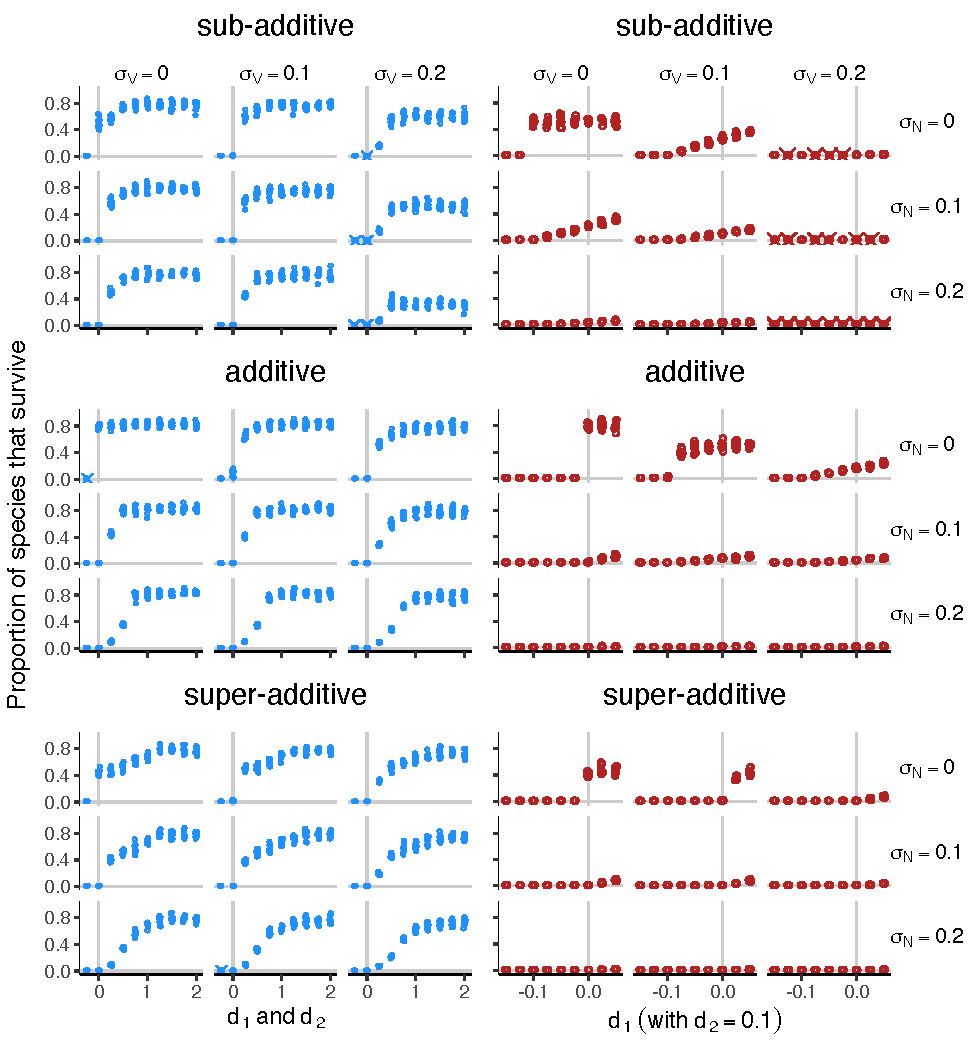
\includegraphics[width=0.9\textwidth]{S3-stoch_coexist.pdf}
\caption{Proportion of species that survived in simulations of 100-species, 2-axis
    communities with
    (A) varying $d_1$ and $d_2$ or 
    (B) varying just $d_1$ with $d_2$ fixed at 0.1.
    Standard deviations are for stochasticity in
    population dynamics ($\sigma_N$) and
    axis evolution ($\sigma_V$).
    Shown for sub-additive ($\eta < 0$), additive ($\eta = 0$), and 
    super-additive ($\eta > 0$) tradeoffs.
    Additive genetic variance ($\sigma_i^2$) was fixed at 0.05 for 
    these simulations.}
\label{fig:stoch-coexist-nspp}
\end{figure}



\begin{figure}[ht!]
\centering
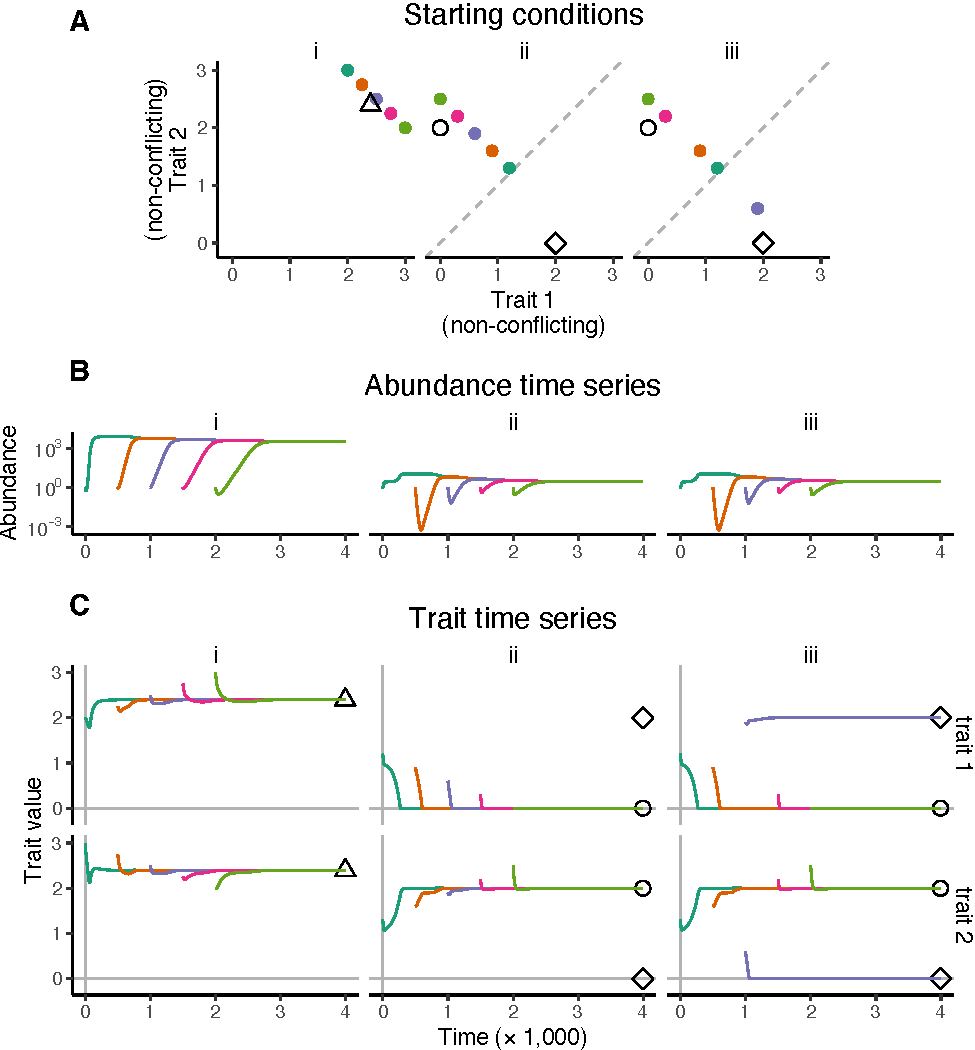
\includegraphics[width=0.7\textwidth]{S1-cond_coexist_non-conflicting.pdf}
\caption{Coexistence for 2-axis, 5-species communities when
    both axes have non-conflicting evolution.
    Panels show, for each of five situations,
    (A) starting conditions and trajectories for each species in axis space, 
    (B) abundances through time, and 
    (C) axis values through time.
    Situation i has sub-additive tradeoffs, situations ii and iv have 
    super-additive, and iii and v have additive.
    (A) Dashed arcs show the location of neutrally stable rings
    when tradeoffs are additive, and 
    the dotted lines separate the basins of attraction for the two possible
    axis states when tradeoffs are super-additive.
    (A,C) Shapes of hollow points indicate the equilibrium axis state.
    (C) For situations iii and v, line width is proportional to the 
    distance from the neutrally stable ring.}
\label{fig:cond-coexist-non-conflicting}
\end{figure}


\begin{figure}[ht!]
\centering
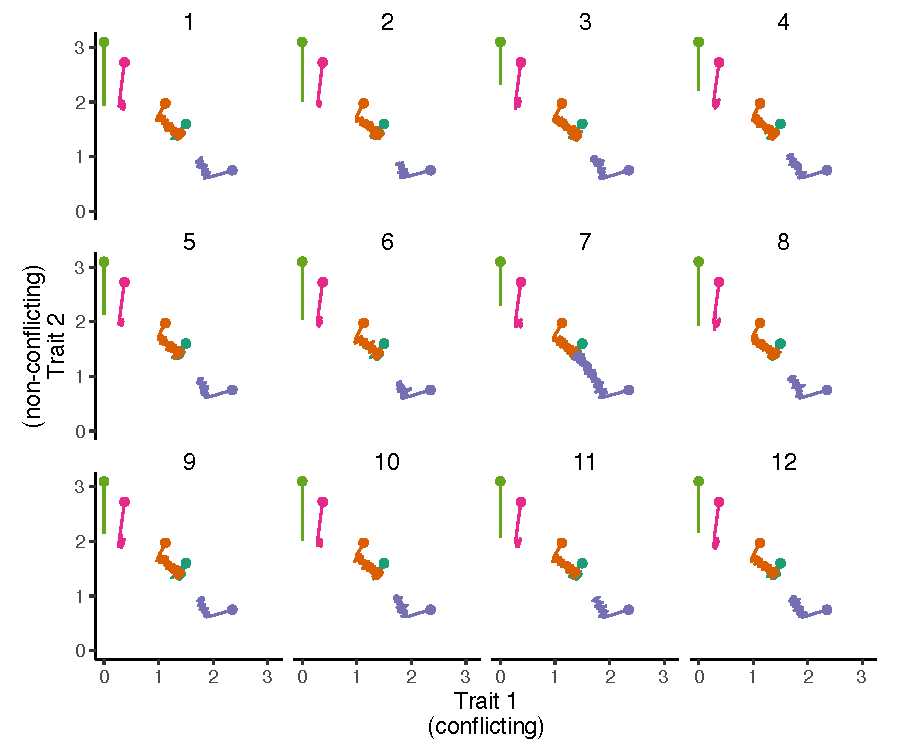
\includegraphics{S2-cc_sigmaV_sit_v.pdf}
\caption{Genotype trajectories through axis space for 12 repetitions under 
scenario v (see main text), with axis stochasticity ($\sigma_V = 0.1$).
Points indicate starting locations, and color indicates species.}
\label{fig:cond-coexist-Vstoch-sit-v}
\end{figure}



\begin{figure}[ht!]
\centering
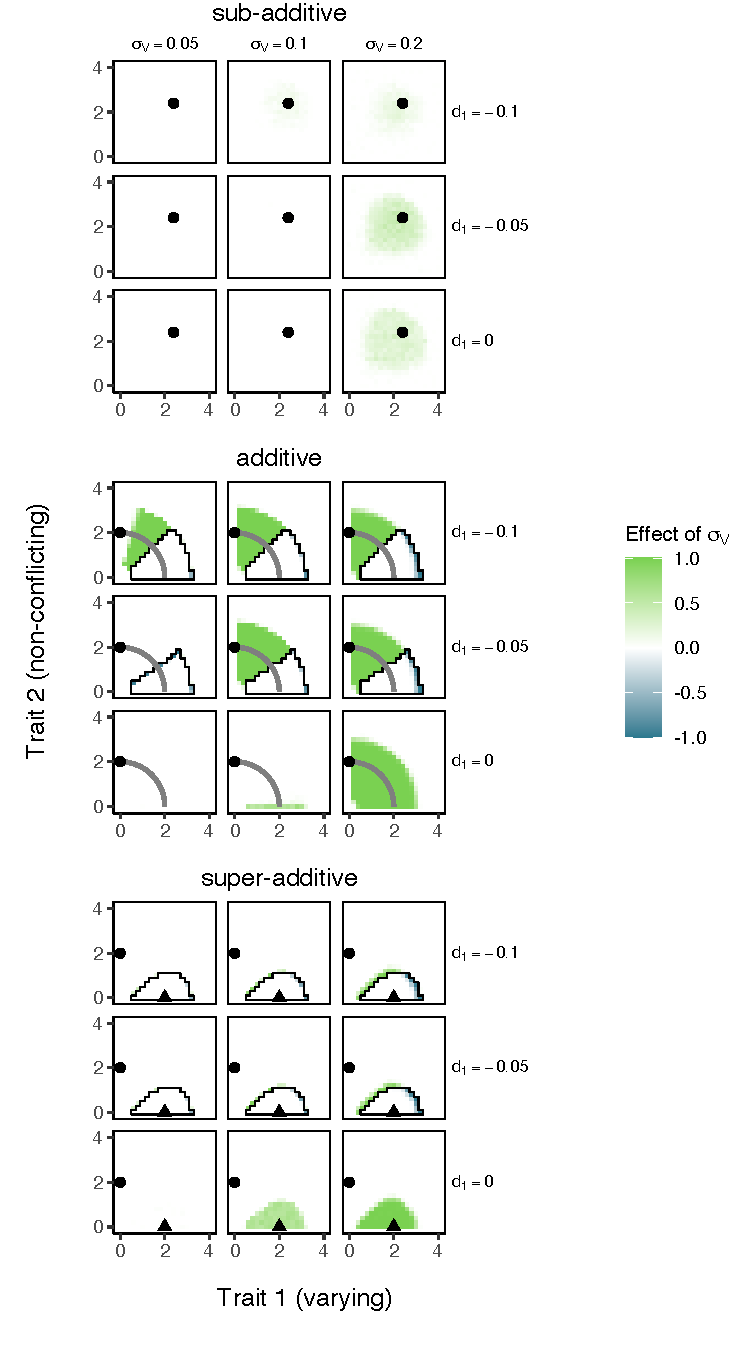
\includegraphics[width=0.5\textwidth]{S4-inv_sims_hm_replace.pdf}
\caption{Effect of stochasticity on replacement of resident species by invader
    based on the invader's starting axis values (x and y axes),
    magnitude of stochasticity (sub-panel columns), and 
    value of $d_1$ (sub-panel rows).
    Shown for sub-additive, additive, and super-additive tradeoffs.}
\label{fig:inv-sims-heatmap-replace}
\end{figure}

\begin{figure}[ht!]
\centering
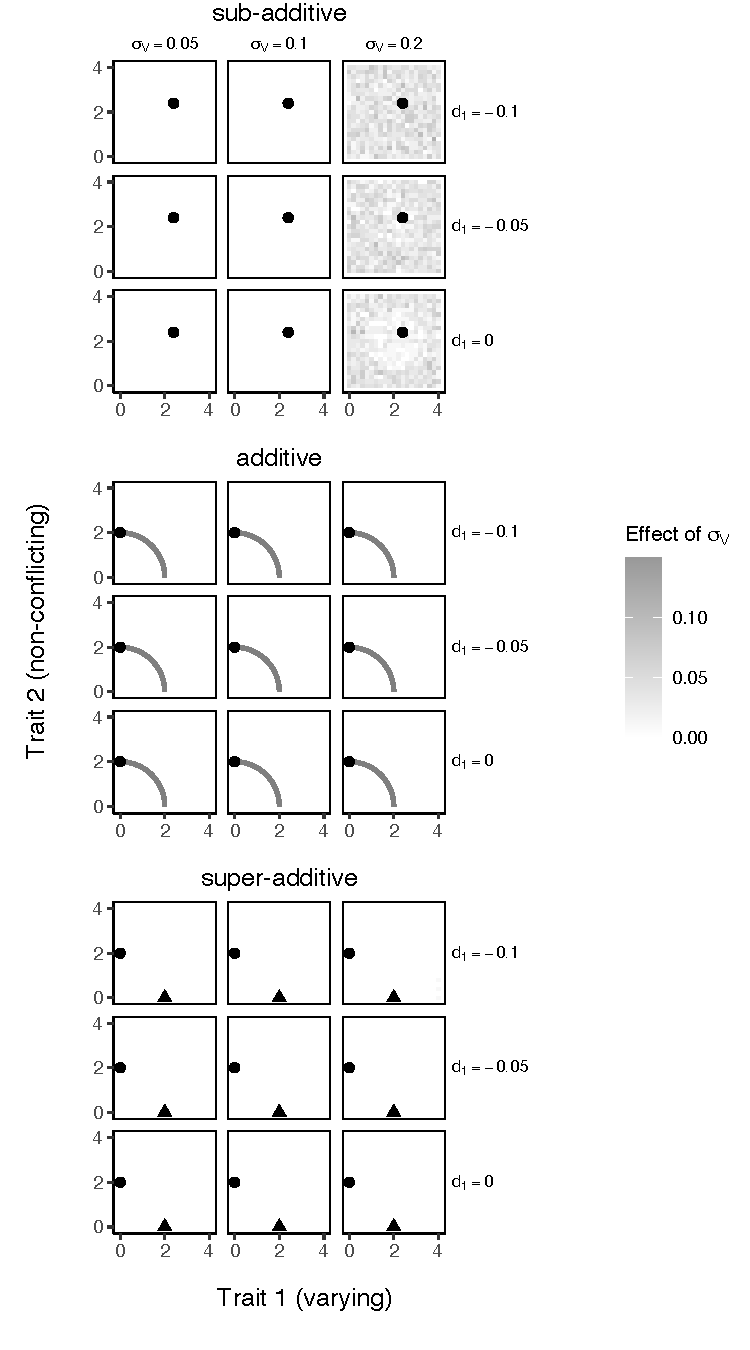
\includegraphics[width=0.5\textwidth]{S5-inv_sims_hm_extinct.pdf}
\caption{Effect of stochasticity on extinction of both resident and invader
    species based on the invader's starting axis values (x and y axes),
    magnitude of stochasticity (sub-panel columns), and 
    value of $d_1$ (sub-panel rows).
    Shown for sub-additive, additive, and super-additive tradeoffs.}
\label{fig:inv-sims-heatmap-extinct}
\end{figure}

